\makeatletter
\makeatother
\documentclass[../main.tex]{subfiles}

\graphicspath{
    {img}
	{../img/}
}

\begin{document}
\section{Метод Римана для решения обобщённой задачи Коши для гиперболического уравнения}

Рассмотрим уравнение гиперболического типа в общей постановке:
\begin{gather}
    \label{eq:2.7.1}
    \pderivtwo{u}{x}{y} + a(x,y)\pderiv{u}{x} +b(x,y)\pderiv{u}{y} + c(x,y)u = f(x,y)\\
    \label{eq:2.7.2}
    u|_{y=g(x)} = \varphi(x)\\
    \pderiv{u}{y}|_{y=g(x)} = \psi(x)
\end{gather}
Выберем точку с координатами $(x_0,y_0)$ и проведём через них прямые,
параллельные осям, причём $y=g(x)$ пересекает прямые $x=x_0$, $y=y_0$ только в одной точке.

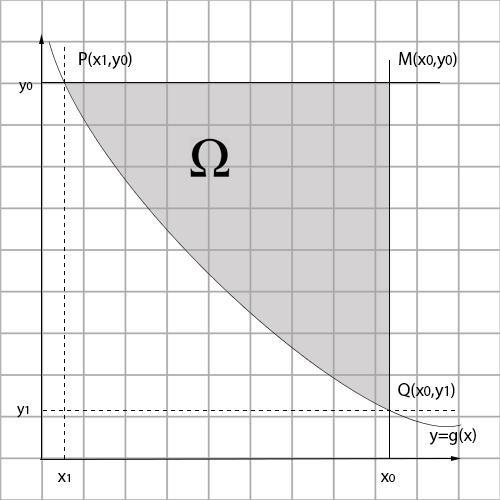
\includegraphics[scale=0.6]{2.7_graph.jpg}    
\\
Область между $y=g(x), x=x_0, y=y_0$ -- $\Omega$\\
$\varphi \in C^2[x_1; x_0], \: \psi \in C^1[x_1,x_0]$\\
\\
Введём дифференциальный оператор $Lu$ и сопряжённый к нему $L^*v$:
$$ Lu = \pderivtwo{u}{x}{y} + a\pderiv{u}{x} +b\pderiv{u}{y} + cu $$
$$ L^*v = \pderivtwo{v}{x}{y} -\pderiv{ }{x}(av) -\pderiv{ }{y}(bv) + cv $$
Так как опреторы сопряжённые, то $vLu - uL^*v$ можно представить в виде
суммы производных по $x$ и $y$ от некоторых функций.
\begin{gather*}
    vLu - uL^*v =
    v(\pderivtwo{u}{x}{y} + a\pderiv{u}{x} +b\pderiv{u}{y} + cu) -
    u(\pderivtwo{v}{x}{y} -\pderiv{ }{x}(av) -\pderiv{ }{y}(bv) + cv) =\\
    = v\pderivtwo{u}{x}{y} + av\pderiv{u}{x} +bv\pderiv{u}{y} + cvu -
    u\pderivtwo{v}{x}{y} +u\pderiv{ }{x}(av) +u\pderiv{ }{y}(bv) - cuv = \\
    =\frac{1}{2} \pderiv{ }{x} \left( v\pderiv{u}{y} - u\pderiv{v}{y} + 2auv\right) + 
    \frac{1}{2} \pderiv{ }{y} \left( v\pderiv{u}{x} - u\pderiv{v}{x} + 2buv\right) =\\
    = \pderiv{H}{x}+\pderiv{K}{y}
\end{gather*}
\begin{equation}
    \label{eq:2.7.3}
    vLu - uL^*v = \pderiv{H}{x}+\pderiv{K}{y},
\end{equation}
где
\begin{equation}
    \label{eq:2.7.4}
    H = \frac{1}{2} \left( v\pderiv{u}{y} - u\pderiv{v}{y} + 2auv\right), \quad
    K = \frac{1}{2}\left( v\pderiv{u}{x} - u\pderiv{v}{x} + 2buv\right)
\end{equation}

\begin{gather*}
    \iint\limits_{\Omega} \left(vLu -uL^*v\right)dxdy = \text{[т.Грина]} =\\
     = \int\limits_{\partial\Omega} -Kdx + Hdy = 
    \int\limits_M^P -Kdx+Hdy + \int\limits_P^Q -Kdx+Hdy + \int\limits_Q^M -Kdx+Hdy = \\
    = I_1+I_2+I_3
\end{gather*}

\begin{gather*}
    I_1 = \int\limits_M^P -Kdx+Hdy = \text{[y не изменяется вдоль МР]} = 
    - \int\limits_M^P Kdx =
    -\frac{1}{2} \int\limits_M^P \left( v\pderiv{u}{x} - u\pderiv{v}{x} + 2buv\right)dx =\\=
    \left[\pderiv{(uv)}{x} = v\pderiv{u}{x} + u\pderiv{v}{x} \right] =
    -\frac{1}{2} \int\limits_M^P \left( \pderiv{(uv)}{x} - 2u\pderiv{v}{x} + 2buv\right)dx =\\=
    -\frac{1}{2}(uv)|_M^P + \int\limits_M^P u(\pderiv{v}{x}-bv)dx
\end{gather*}

\begin{gather*}
    I_3 = \frac{1}{2}(uv)|_Q^M - \int\limits_Q^M u(\pderiv{v}{y}-av)dy
\end{gather*}

Тогда:
\begin{gather*}
    I_1+I_2+I_3 = 
    -\frac{1}{2}(uv)|_M^P + \int\limits_M^P u(\pderiv{v}{x}-bv)dx + 
    \int\limits_P^Q -Kdx+Hdy +
    \frac{1}{2}(uv)|_Q^M - \int\limits_Q^M u(\pderiv{v}{y}-av)dy
\end{gather*}

Выберем $v$ таким образом, что:
\begin{enumerate}
    \item $L^*v = 0$
    \item $\pderiv{v}{x}-bv|_{y=y_0} = 0$
    \item $\pderiv{v}{y}-av|_{x=x_0} = 0$
\end{enumerate}

\begin{gather*}
    \pderiv{v}{x}-bv|_{y=y_0} = 0\\
    \frac{dv(x,y_0)}{v} = b(x,y_0)dx\\
    \log v|_{x_0}^x = \int\limits_{x_0}^x b(x,y_0)dx\\
\end{gather*}
Введём условие $v(x_0,y_0)=1$ -- \textit{условие согласованности}. Тогда:
\begin{gather}
    \label{eq:2.7.5}
    v|_{y=y_0} = e^{\int\limits_{x_0}^x b(x,y_0)dx}\\
    \label{eq:2.7.6}
    v|_{x=x_0} = e^{\int\limits_{y_0}^y a(x_0,y)dy}
\end{gather}
\\
Получим \textbf{задачу Гурса}:
\begin{equation}
    \begin{gathered}
        \label{eq:2.7.7}
        L^*v=0\\
        v|_{y=y_0} = e^{\int\limits_{x_0}^x b(x,y_0)dx}\\
        v|_{x=x_0} = e^{\int\limits_{y_0}^y a(x_0,y)dy}\\
        v(x_0,y_0)=1
    \end{gathered}
\end{equation}
Условия заданы на характеристиках. Имеет единственное решение.
\\
$v$ -- решение (\ref{eq:2.7.7}) -- называется \textbf{функцией Римана}
\\
$Lu=f$ по условию. Вернёмся к (\ref{eq:2.7.3}). $L^*v=0$, тогда:
\begin{gather*}
    vLu - uL^*v = \iint\limits_{\Omega} vfdxdy =
    -\frac{1}{2}(uv)|_M^P + \frac{1}{2}(uv)|_Q^M + \int\limits_{PQ}-Kdx + Hdy =\\=
    \left[(uv)|_M^P = (uv)|_P - u(x_0, y_0), \quad (uv)|_Q^M = u(x_0, y_0) - (uv)|_Q\right] =\\=
    -\frac{1}{2}(uv)|_P +\frac{1}{2} u(x_0, y_0) + \frac{1}{2} u(x_0, y_0) - \frac{1}{2}(uv)|_Q +
    \int\limits_{PQ}-Kdx+Hdy
\end{gather*}
Получим \textbf{формулу Римана} для решения обобщённой задачи Коши
\begin{equation}
    \begin{gathered}
        \label{eq:2.7.8}
        u(x_0,y_0) = \frac{1}{2}(uv)|_P + \frac{1}{2}(uv)|_Q+\\+
        \frac{1}{2}\int_{PQ}\left(v\pderiv{u}{x} - u\pderiv{v}{x} + 2buv\right)dx +
        \left(v\pderiv{u}{y} - u\pderiv{v}{y} + 2auv\right)dy +
        \iint\limits vfdxdy
    \end{gathered}
\end{equation}
\\
Чтобы решить задачу \textit{методом Римана} необходимо:
\begin{enumerate}
    \item Выписать задачу Гурса (\ref{eq:2.7.7}) 
    \item Найти функцию $v$
    \item По формуле (\ref*{eq:2.7.8}) построить решеиние исходной задачи
\end{enumerate}
\textit{Замечание 1:} Решение в точке $M$ определяет характеристический треугольник $MPQ$\\
\\
\textit{Замечание 2:} Характеристики персекают функцию $g(x)$ только в одной точке.
Если они пересекают в двух точках, например $P_1, P_2, Q$, то решение в точке $M$ 
определяли бы два треугольника -- $MP_1Q$ и $MP_2Q$, т.е. решеиние былобы не единственным.
\end{document}